% !TEX spellcheck = uk_en
\documentclass[main.tex]{subfiles} 

\begin{document}

\section{Undervisningsopplegget}
\label{sec:1}

\textbf{Kompetansemål i læreplanen}
\newline
\emph{Forskerspiren} :
\begin{itemize}
\item formulere testbare hypoteser, planlegge og gjennomføre undersøkelser 
av dem og diskutere observasjoner og resultater i en rapport
\end{itemize}
\emph{Mangfold i naturen} :
\begin{itemize}
\item beskrive oppbygningen av dyre- og planteceller og forklare hovedtrekkene i fotosyntese og celleånding
\item gjøre rede for celledeling og for genetisk variasjon og arv
\end{itemize}
Dette opplegget utførte jeg alene, med veileder og en medstudent som observatører. 
De bidro også med å gi personlig/gruppe veiledning når elevene jobbet enten selvstendig eller i grupper. 
Undervisningseksvensene er fordelt over 3 skoletimer fordelt over 2 uker. Opplegget ble laget i henhold til 
forutsetningene til elevene og deres bakgrunn. 

Vi observerte elevene i både naturfagtimer og mattetimer. Elevenes faglig bakgrunn er varierende. Før 
undervisningsopplegget var utført observerte vi elevene i en naturfag time der de brukte mikroskop til å studere 
celleprøver og celler fra deres egen munn. Elevene var fordelt i grupper på 4 stykker, og læreren gikk rundt og 
veiledet alle gruppene, deriblant hjalp læreren med å innstille mikroskopene til elevene slik at de endte opp med
riktig fokus. Læreren gjennomgikk deretter felles med elevene med sitt eget mikroskop
som var koblet til datamaskinen. Bildet fra mikroskopet ble projisjert på lystavlen i laboratoriet. Dette inspirerte 
oss til å bruke en tilsvarende opplegg til å strukturere vår egen undervisningstime(r).

\subsection{OneNote}

\begin{figure}[h!]
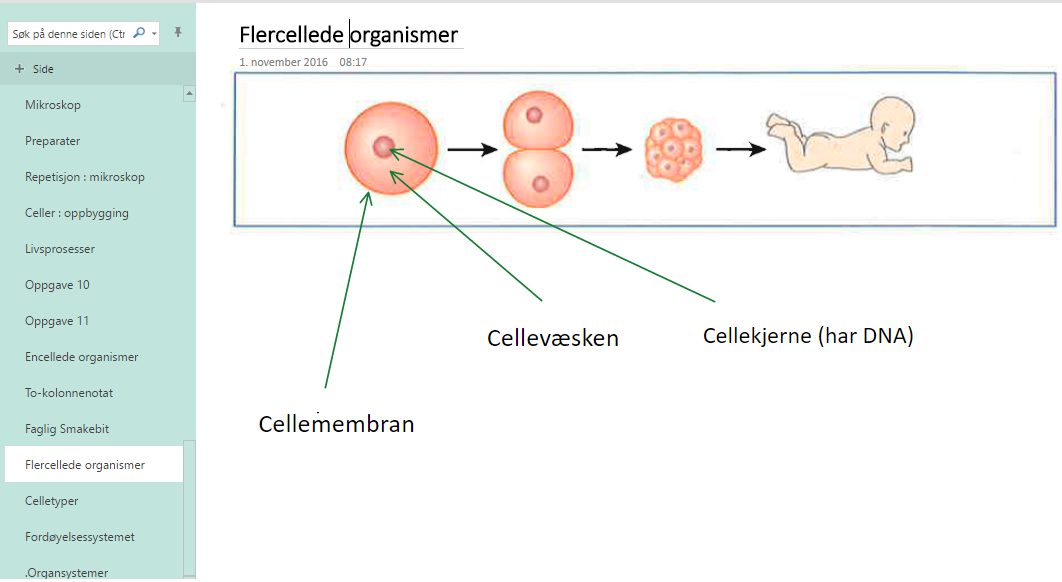
\includegraphics[scale = 0.6]{../figures/onenote_flercellet.png}
\caption{Notat 1}
\end{figure}

\begin{figure}[h!]
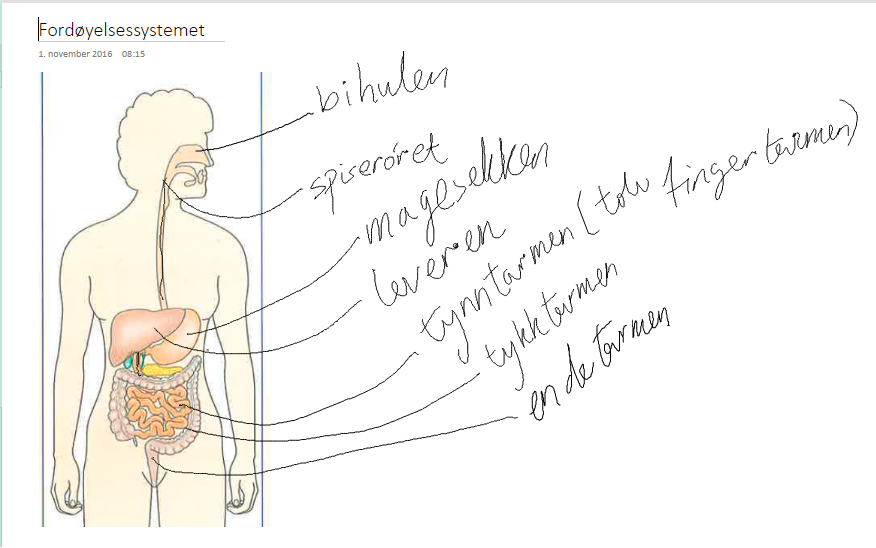
\includegraphics[scale = 0.6]{../figures/onenote_fordoyelse.png}
\caption{Notat 2}
\end{figure}

\subsection{1.time}

\subsection{2.time}

\subsection{3.time}

\end{document}
